\documentclass[conference]{IEEEtran}

\usepackage{cite}
\usepackage{amsmath,amssymb,amsfonts}
\usepackage{algorithmic}
\usepackage{graphicx}
\usepackage{textcomp}
\usepackage{xcolor}
\def\BibTeX{{\rm B\kern-.05em{\sc i\kern-.025em b}\kern-.08em
		T\kern-.1667em\lower.7ex\hbox{E}\kern-.125emX}}

\begin{document}
	\title{Implementing the Bayes Classifier for Linearly Separable Multivariate Data\\
		\thanks{Identify applicable funding agency here. If none, delete this.}
	}
	
	\author{\IEEEauthorblockN{Pawan Ram Mali (PhD)}
		\IEEEauthorblockA{\textit{Department of CSE } \\
			\textit{Indian Institute of Technology}\\
			Dharwad, India \\
			cs24dp011@iitdh.ac.in}
		\and
		\IEEEauthorblockN{Sachin Maurya (MS)}
		\IEEEauthorblockA{\textit{Department of CSE} \\
			\textit{Indian Institute of Technology}\\
			Dharwad, India \\
			cs24ms002@iitdh.ac.in}
		\and
		\IEEEauthorblockN{Abhishek Sharma (MS)}
		\IEEEauthorblockA{\textit{Department of CSE} \\
			\textit{Indian Institute of Technology}\\
			Dharwad, India \\
			cs24ms003@iitdh.ac.in}
	}
	
	\maketitle
	
	\begin{abstract}
		\\
		This project delves into the implementation of a **Bayesian classifier** using multivariate Gaussian distributions to classify data points into one of three distinct classes. The classifier computes posterior probabilities based on Bayes' theorem and is evaluated using various statistical metrics. Additionally, decision boundaries are visualized to demonstrate the model's effectiveness in separating the feature space into distinct regions corresponding to the classes. Through rigorous evaluation, this project highlights the strengths of the Bayesian classifier in statistical pattern recognition.
		
		We provide hands-on experience in developing, evaluating, and visualizing a Bayesian classifier, while also reinforcing theoretical concepts such as Gaussian distribution assumptions, class priors, and posterior probability calculations.
	\end{abstract}
	
	\section{Introduction}
	
	The **Bayesian classifier** is a powerful tool in statistical pattern recognition. In this project, we use it to classify data points into one of three classes based on their features. Each class is assumed to follow a multivariate Gaussian distribution. The classifier calculates the posterior probability for each class and assigns data points to the class with the highest posterior.
	
	This project aims to:
	- Implement a Bayesian classifier using multivariate Gaussian distributions.
	- Evaluate the classifier's performance with metrics such as accuracy, precision, recall, and F1-score.
	- Visualize the decision boundaries that separate the classes, providing insight into the classifier's behavior.
	
	The classifier is tested on a dataset where each class is represented by two features. Through analysis and visualization, we assess how well the classifier distinguishes between classes.
	
	\[
	P(C_k \mid x) = \frac{P(x \mid C_k) \cdot P(C_k)}{P(x)}
	\]
	
	\begin{itemize}
		\item \textbf{Posterior Probability} \( P(C_k \mid x) \): Probability of class \( C_k \) given the observed data \( x \).
		\item \textbf{Prior Probability} \( P(C_k) \): Initial belief about class \( C_k \) before observing the data.
		\item \textbf{Likelihood} \( P(x \mid C_k) \): Probability of observing data \( x \) given that the class is \( C_k \).
		\item \textbf{Evidence} \( P(x) \): Normalizing constant ensuring the sum of posterior probabilities equals 1.
	\end{itemize}
	
	\section{Objectives}
	
	The key objectives of this project are:
	
	\begin{enumerate}
		\item \textbf{Classifier Development:} Build a Bayesian classifier based on multivariate Gaussian distributions for three classes of data.
		\item \textbf{Model Evaluation:} Use statistical metrics such as confusion matrix, accuracy, precision, recall, and F1-score to evaluate the classifier’s performance.
		\item \textbf{Decision Boundary Visualization:} Visualize the decision boundaries that separate the different classes, allowing for a clear understanding of how the classifier behaves.
	\end{enumerate}
	
	\section{Exploratory Data Analysis (EDA)}
	
	Before implementing the classifier, it is essential to explore and understand the data. We load the data, which consists of three classes, each with two features. Using scatter plots, we can observe how each class is distributed and identify any overlap or separability.
	
	\subsection{Data Distribution}
	Distribution plots are used to visualize the distribution of the data points for each class in the feature space. This helps identify any overlaps or separability between classes.
	
	\begin{figure}[h!]
		\centering
		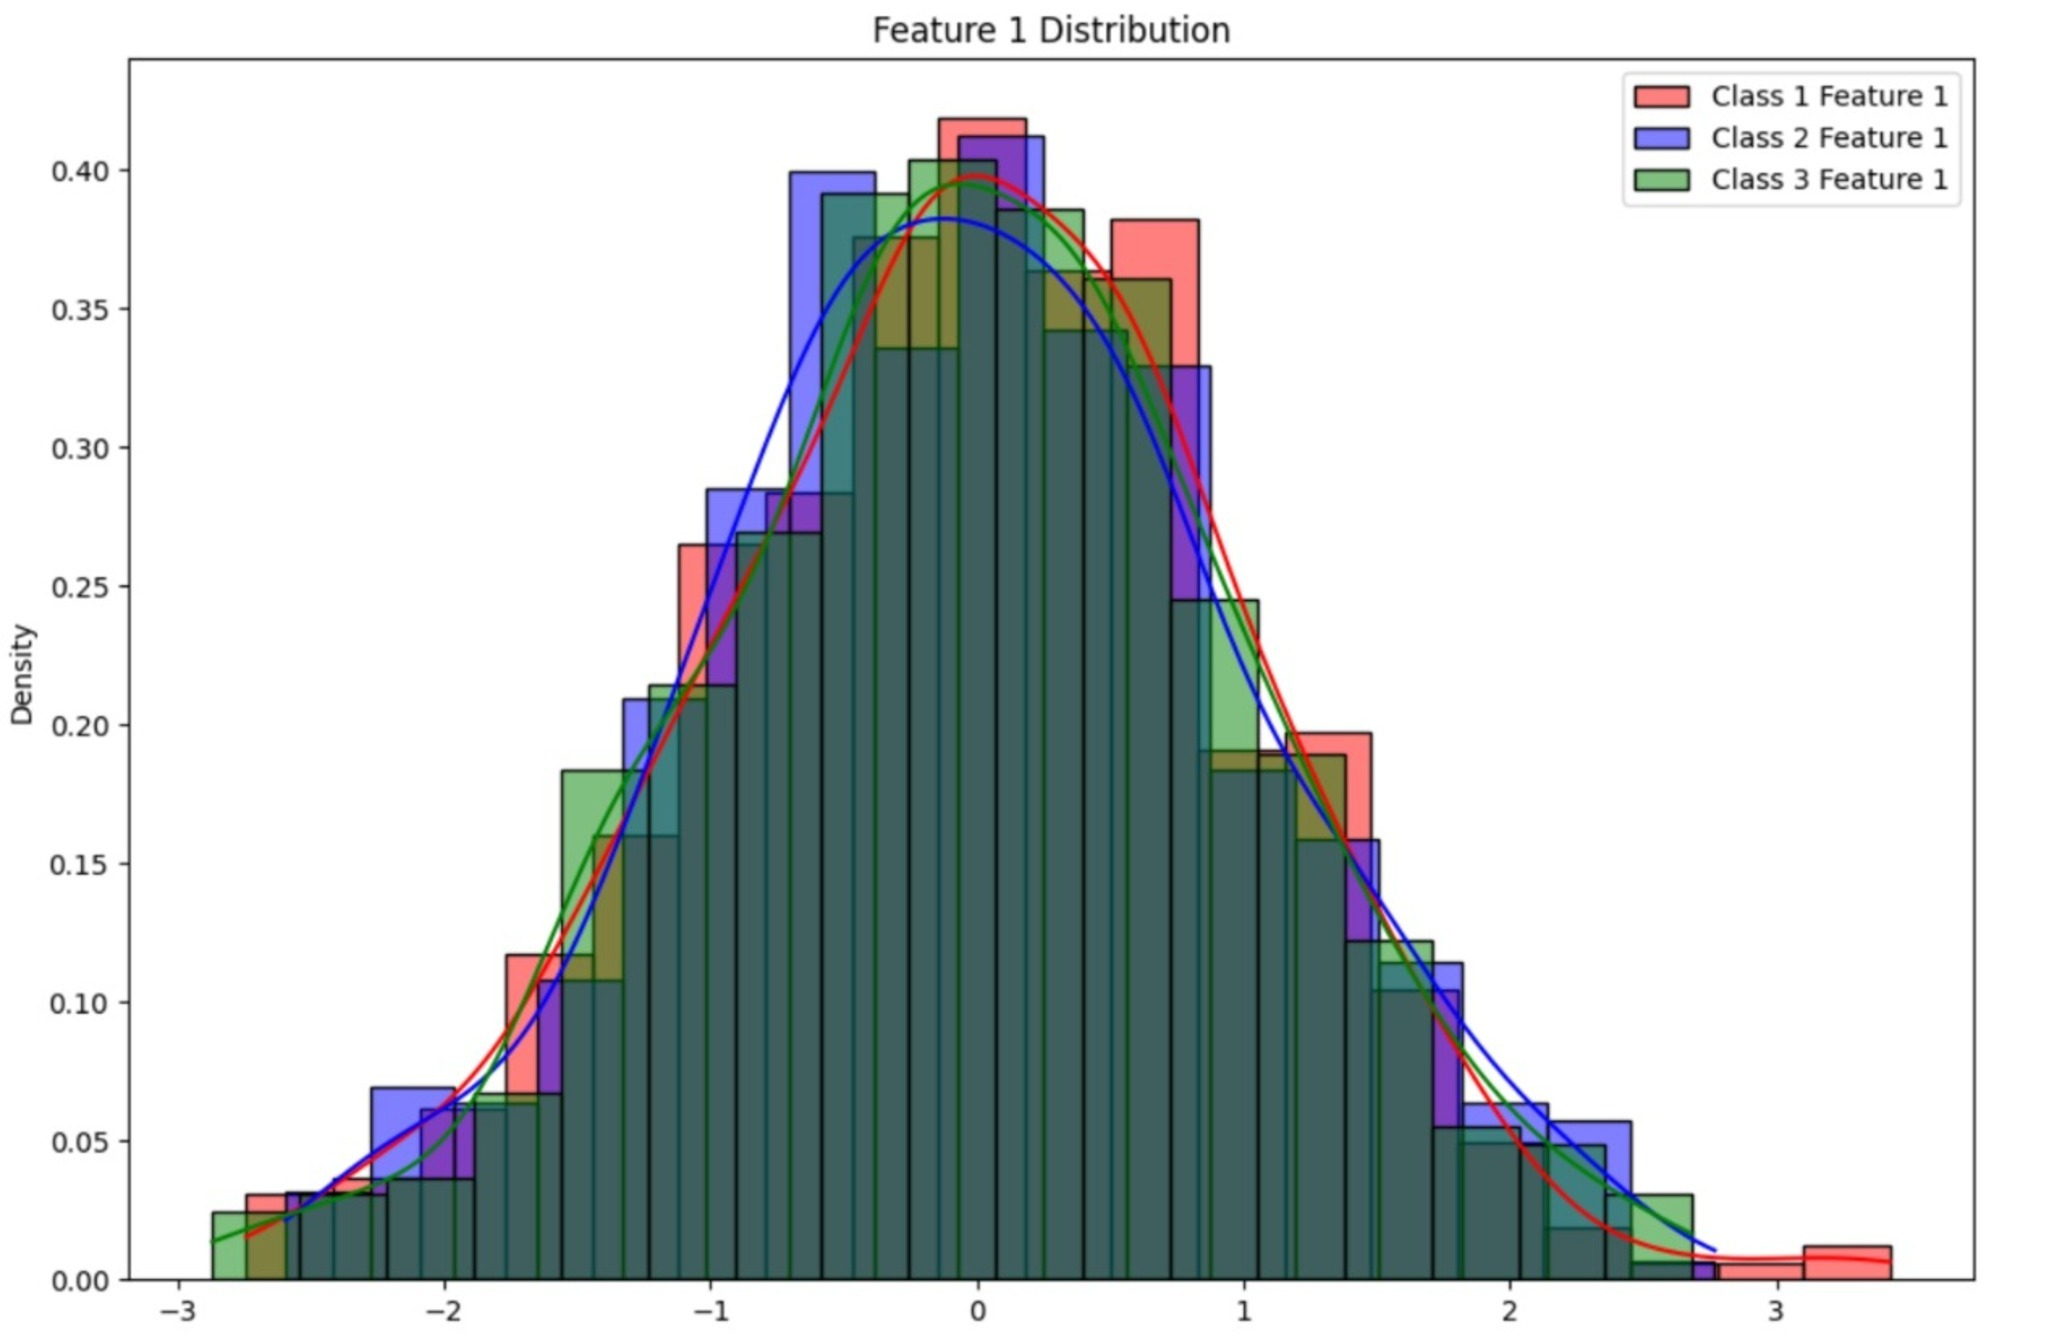
\includegraphics[width=0.5\textwidth, height=5cm]{figr1.jpg}
		\caption{Showing class distribution.}
		\label{fig:class_distribution}
	\end{figure}
	
	
	\subsection{Cluster Formation}
	The distribution plots also help reveal any natural clustering of data points within each class, providing insight into the structure of the dataset.
	
	\section{Data Processing}
	
	The data is preprocessed to ensure it is suitable for the Bayesian classifier. This involves several key steps:
	
	\subsection{Normalization/Standardization}
	The data is standardized to have zero mean and unit variance to ensure that the features are on a comparable scale.
	
	\subsection{Data Splitting}
	The dataset is split into training and testing sets to evaluate the classifier's performance. The training set is used to build the model, while the test set is used for evaluation.
	
	\begin{figure}[h!]
		\centering
		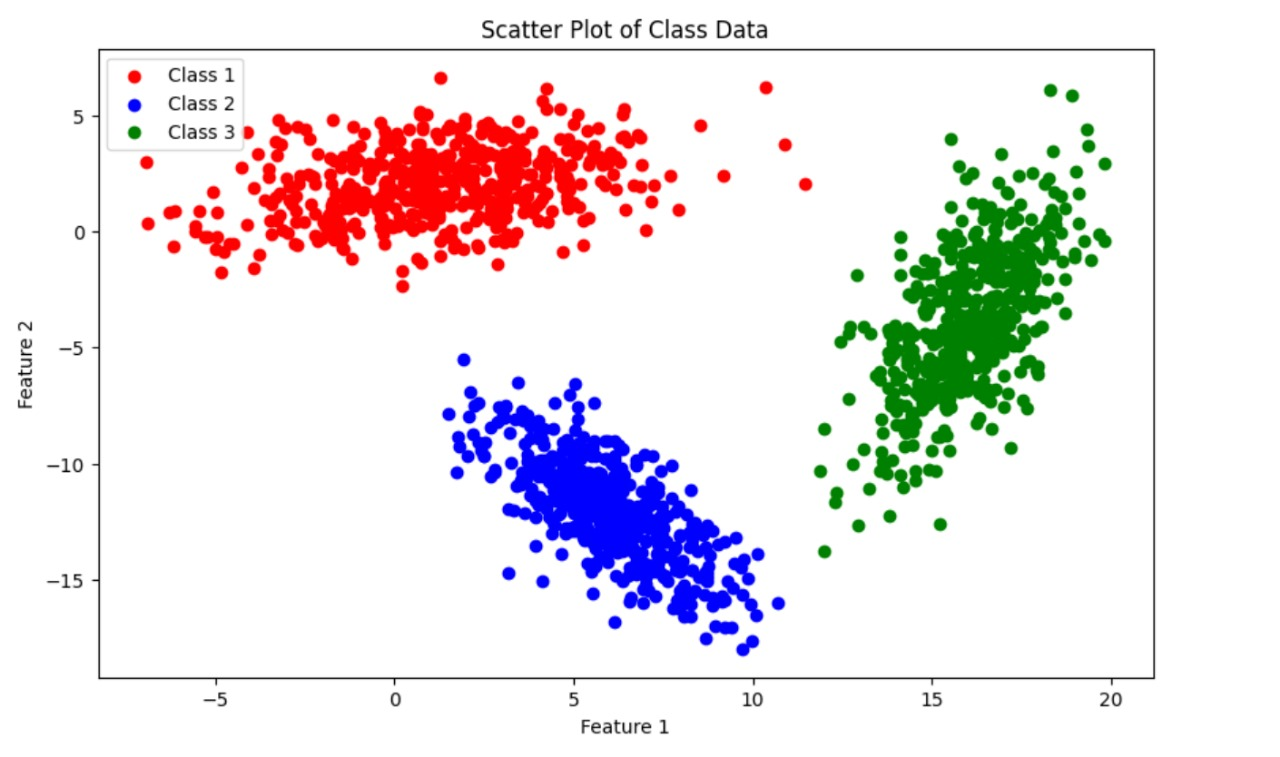
\includegraphics[width=0.5\textwidth, height=5cm]{figr2.jpg}
		\caption{Visualization of data splitting between training and testing sets.}
		\label{fig:data_splitting}
	\end{figure}

	
	\section{Bayesian Classifier}
	
	\subsection{Multivariate Gaussian Distribution}
	We compute the mean and covariance matrix for each class. The classifier assumes that the data follows a multivariate Gaussian distribution, which is characterized by the following probability density function:
	
	\[
	f(x; \mu, \Sigma) = \frac{1}{(2\pi)^{d/2} |\Sigma|^{1/2}} \exp\left(-\frac{1}{2} (x - \mu)^T \Sigma^{-1} (x - \mu)\right)
	\]
	
	where:
	\begin{itemize}
		\item \( x \) is the data point,
		\item \( \mu \) is the mean vector,
		\item \( \Sigma \) is the covariance matrix.
	\end{itemize}
	
	\subsection{Posterior Calculation}
	The posterior probability for each class is calculated using Bayes' theorem. The class with the highest posterior is assigned to the data point.
	
	\section{Diagonal Covariance Matrix}
	In this scenario, the covariance matrix for each class is diagonal, meaning that the off-diagonal elements, which represent correlations between different features, are zero. The diagonal elements represent the variances of each feature. This assumption simplifies the model as it reduces the number of parameters to be estimated, making it computationally more efficient. This approach assumes that the features are uncorrelated with each other within each class.
	
	The probability density function for a multivariate Gaussian distribution with a diagonal covariance matrix is given by:
	
	\[
	f(x; \mu, \Sigma) = \frac{1}{(2\pi)^{d/2} |\Sigma|^{1/2}} \exp\left(-\frac{1}{2} (x - \mu)^T \Sigma^{-1} (x - \mu)\right)
	\]
	
	where \( \Sigma \) is a diagonal matrix specific to each class.
	
	\section{Shared Full Covariance Matrix}
	In this case, all classes share the same full covariance matrix, denoted as \( \Sigma \). This assumption implies that the shapes of the distributions for different classes are identical, though their centers (means) might differ. The covariance matrix \( \Sigma \) contains non-zero off-diagonal elements, allowing the model to capture correlations between features across all classes.
	
	The probability density function for this scenario is:
	
	\[
	f(x; \mu_k, \Sigma) = \frac{1}{(2\pi)^{d/2} |\Sigma|^{1/2}} \exp\left(-\frac{1}{2} (x - \mu_k)^T \Sigma^{-1} (x - \mu_k)\right)
	\]
	
	where the covariance matrix \( \Sigma \) is shared across all classes, simplifying the model by assuming similar variances and covariances for all classes.
	
	\section{Diagonal Covariance Matrix for Each Class}
	Under this assumption, the covariance matrix is diagonal, but each class has its own distinct diagonal matrix. This means that while the features are uncorrelated within each class, the variances of the features differ from class to class. The diagonal elements of the covariance matrix represent the variance of each feature, and these variances can vary across classes.
	
	The probability density function for each class is:
	
	\[
	f(x; \mu_k, \Sigma_k) = \frac{1}{(2\pi)^{d/2} |\Sigma_k|^{1/2}} \exp\left(-\frac{1}{2} (x - \mu_k)^T \Sigma_k^{-1} (x - \mu_k)\right)
	\]
	
	where \( \Sigma_k \) is the diagonal covariance matrix specific to class \( k \).
	
	\section{Full Covariance Matrix for Each Class}
	In this approach, each class has its own full covariance matrix \( \Sigma_k \), which allows the model to capture the specific correlations between features for each class. This is the most flexible and general form of the multivariate Gaussian distribution, as it makes no assumptions about the relationships between features being the same across classes.
	
	The probability density function for this model is:
	
	\[
	f(x; \mu_k, \Sigma_k) = \frac{1}{(2\pi)^{d/2} |\Sigma_k|^{1/2}} \exp\left(-\frac{1}{2} (x - \mu_k)^T \Sigma_k^{-1} (x - \mu_k)\right)
	\]
	
	where \( \Sigma_k \) represents the full covariance matrix for class \( k \), capturing unique variances and covariances for each class.
	
	
	
	\section{Model Evaluation}
	
	\subsection{Accuracy}
	The classifier’s accuracy is computed by comparing the predicted labels to the true labels in the test set.
	
	\subsection{Confusion Matrix, Precision, Recall, and F1 Score}
	The confusion matrix provides insight into the true positive, false positive, true negative, and false negative classifications. Precision, recall, and F1 scores are calculated to evaluate the classifier's ability to correctly identify each class.
	
	\begin{figure}[h!]
		\centering
		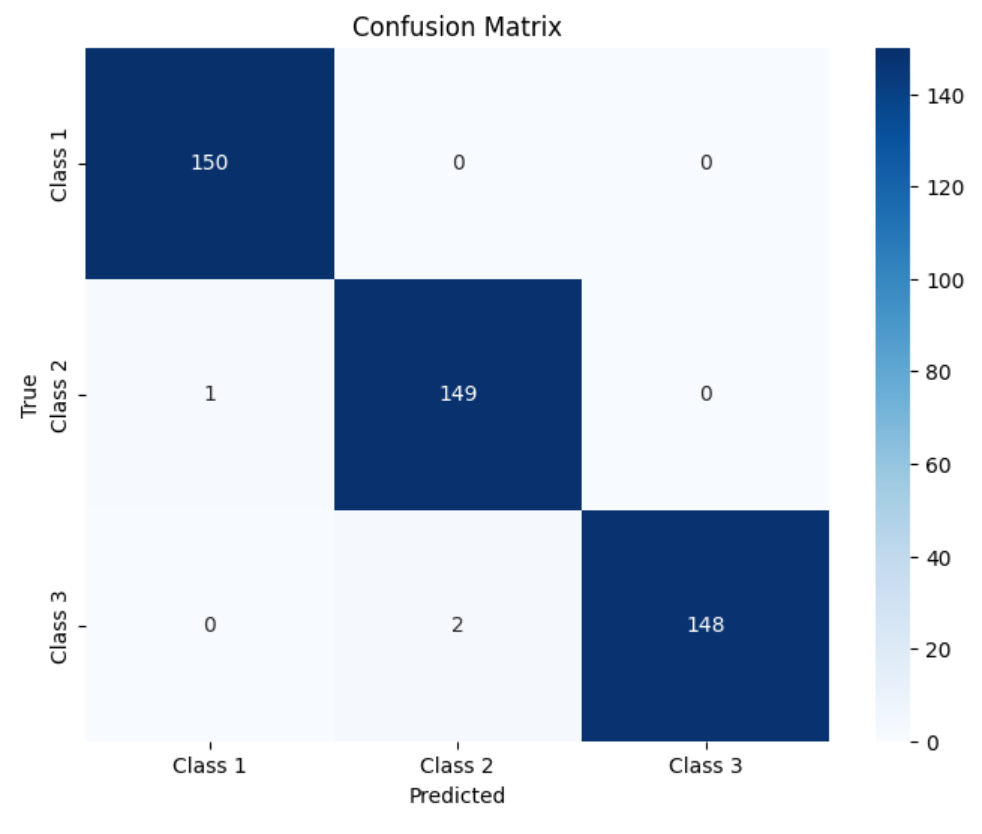
\includegraphics[width=0.5\textwidth, height=5cm]{figr3.png}
		\caption{Confusion matrix visualization}
		\label{fig:decision_region}
	\end{figure}
	
	
	\section{Visualization of Decision Boundaries}
	
	\subsection{Density Contour Plot}
	A density contour plot visualizes the likelihood of data points belonging to each class based on the multivariate Gaussian distributions. It shows how the probability density varies across the feature space.
	
	\begin{figure}[h!]
		\centering
		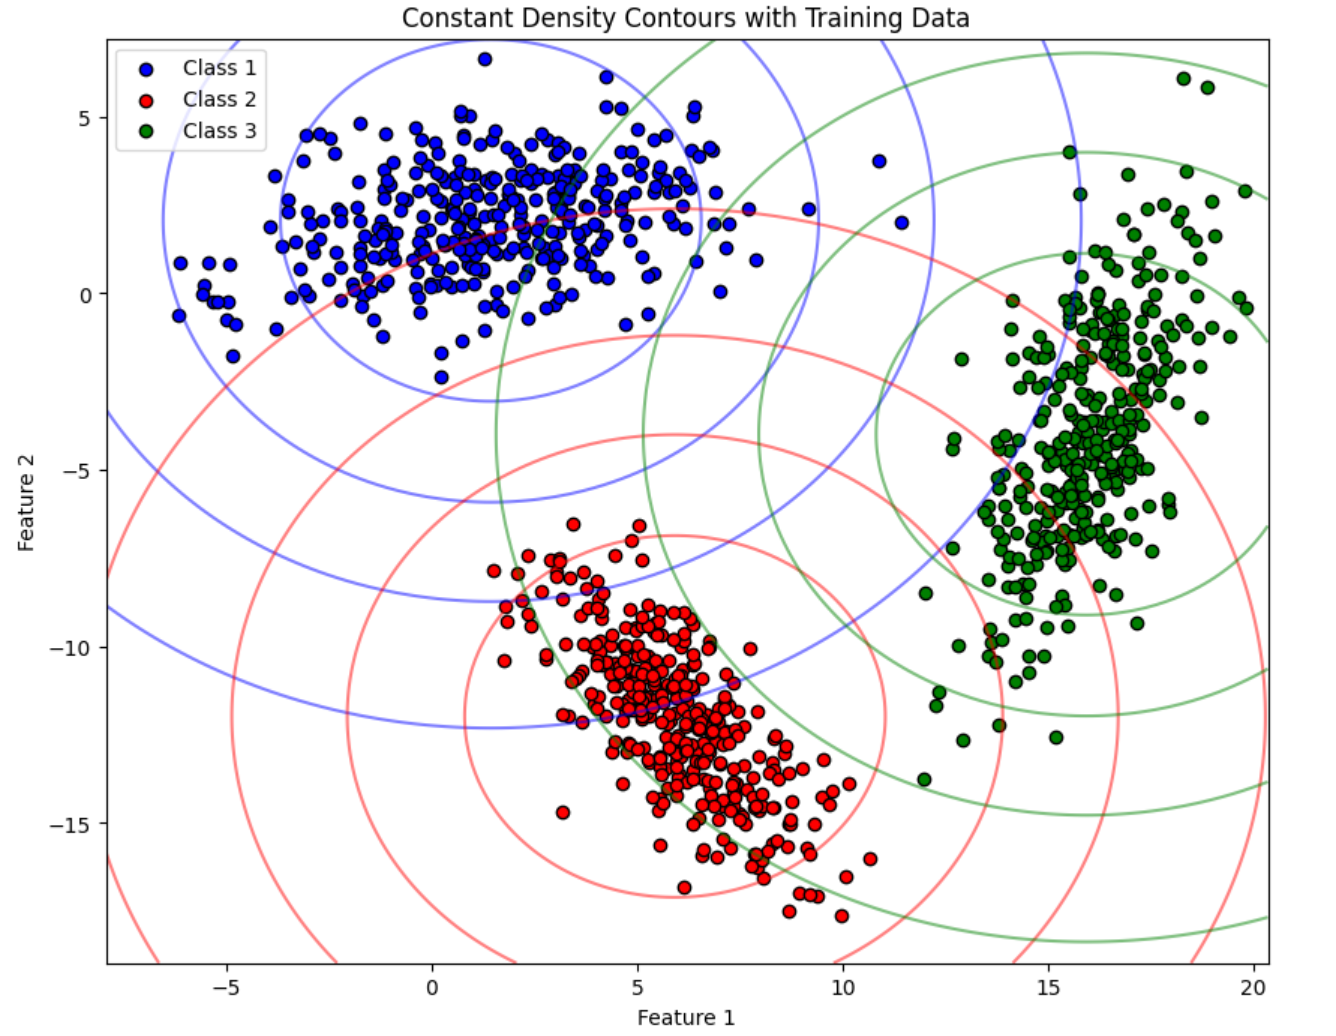
\includegraphics[width=0.5\textwidth, height=5cm]{figr4.png}
		\caption{Density contour plot showing class regions.}
		\label{fig:density_contour}
	\end{figure}

	
	\subsection{Decision Region Plot}
	The decision region plot shows the areas of the feature space where the classifier predicts each class. The training data is overlaid on the plot to demonstrate how well the classifier has learned to separate the classes.
	
	\begin{figure}[h!]
		\centering
		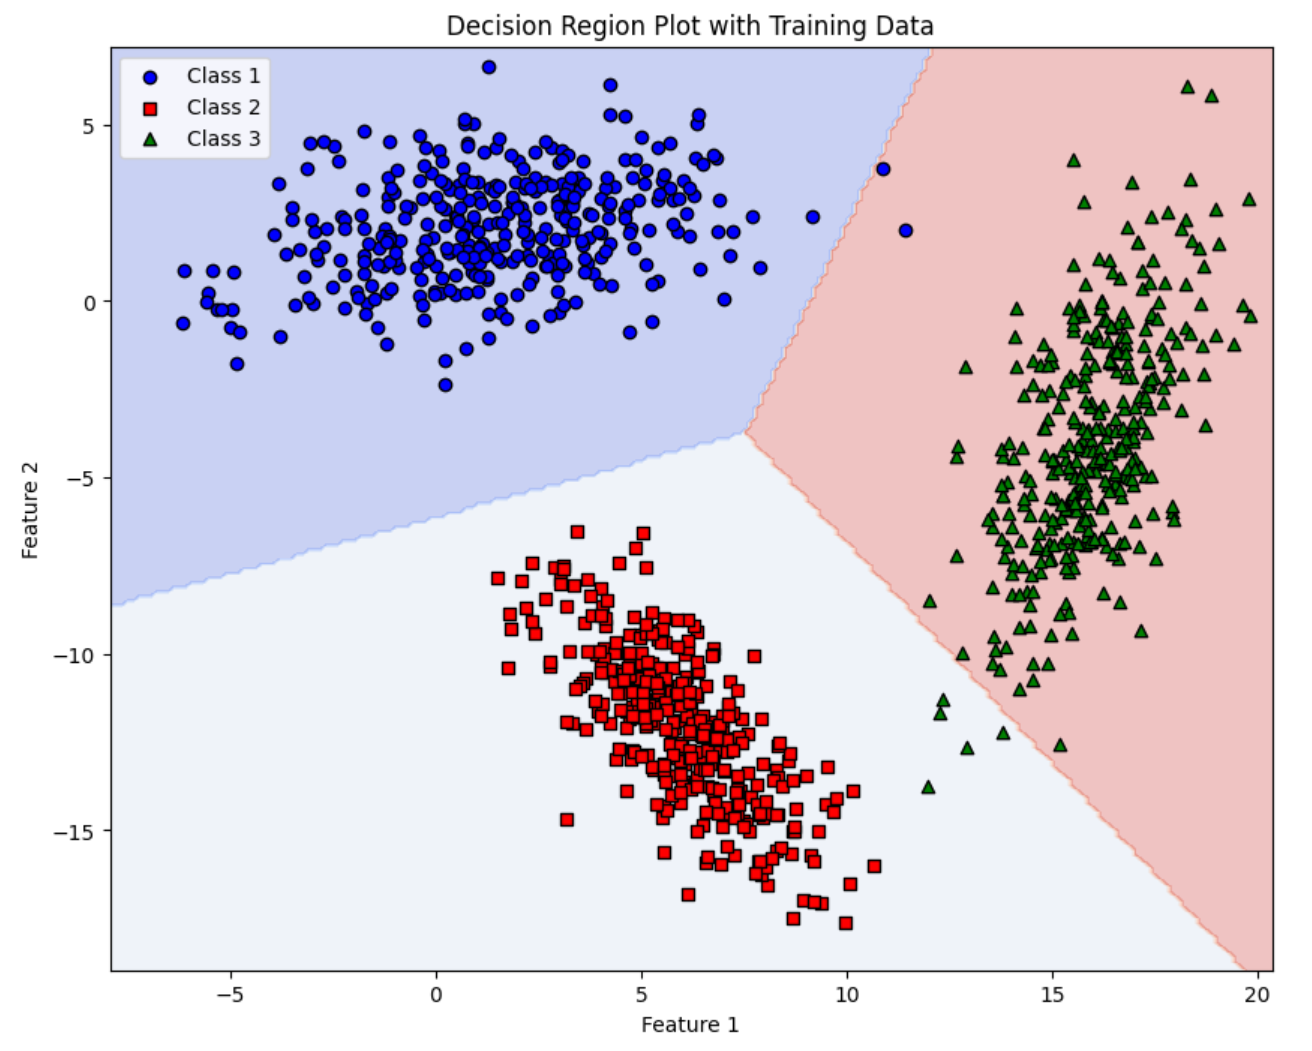
\includegraphics[width=0.5\textwidth, height=5cm]{figr5.png}
		\caption{Decision region plot with training data.}
		\label{fig:decision_region}
	\end{figure}

	
	\section{Conclusion}
	
	The Bayesian classifier was successfully implemented and rigorously tested on a dataset containing three distinct classes. Throughout the process, the classifier demonstrated its effectiveness by accurately predicting the class membership of data points based on their features. The use of multivariate Gaussian distributions for each class allowed the model to capture the underlying patterns and relationships within the data. By leveraging Bayes' theorem, the classifier computed the posterior probabilities for each data point, assigning it to the class with the highest probability.
	
	The results from the evaluation metrics, including accuracy, precision, recall, and F1-score, reflect the model's robust performance in correctly classifying the test data. These metrics confirmed that the Bayesian classifier not only achieved high accuracy but also maintained a balanced performance across all three classes, with minimal misclassification errors.
	
	Moreover, the visualizations of decision boundaries played a critical role in providing a deeper understanding of how the classifier separates the data in the feature space. These visualizations highlighted the regions where each class was dominant and illustrated the boundaries where the classifier transitioned from predicting one class to another. The contour and decision region plots made it evident how well the model captured the complex relationships between features and class membership, offering valuable insights into the classification process.
	
	In conclusion, the combination of theoretical rigor and visual interpretability showcased by the Bayesian classifier makes it an effective tool for pattern recognition, especially in scenarios where class distributions follow a Gaussian pattern. The project's successful implementation and thorough evaluation underscore the classifier’s potential for real-world applications where accurate and interpretable classification is crucial.
	
	Future improvements could include:
	\begin{itemize}
		\item Using class-specific covariance matrices to handle cases with differing variances.
		\item Extending the model to handle higher-dimensional data.
	\end{itemize}
	
	\section*{Acknowledgment}
	
	The completion of this project would not have been possible without the guidance and support of several individuals. First and foremost, we would like to express our deepest gratitude to Dr. Dileep AD, Associate Professor and Head of the Department of Computer Science and Engineering at the Indian Institute of Technology, Dharwad, for his continuous encouragement, insightful feedback, and valuable guidance throughout this project.
	
	We are also incredibly grateful to all the Teaching Assistants who contributed their time and knowledge. Their assistance with technical concepts, problem-solving, and constructive criticism during the various phases of the project was instrumental in its successful completion. Their willingness to help and share their expertise greatly enriched our learning experience.
	
	Finally, we would like to thank the entire faculty and staff of the Department of Computer Science and Engineering at IIT Dharwad for providing us with the resources and a conducive learning environment that made this project possible.
	
	To everyone who contributed to the success of this project, we extend our heartfelt thanks.


	
	\begin{thebibliography}{00}
		
		\bibitem{b1} Duda, R. O., Hart, P. E., \& Stork, D. G. (2000). \textit{Pattern Classification} (2nd ed.). Wiley-Interscience.
		- A comprehensive textbook covering various classification techniques, including Bayes classifiers and decision theory.
		
		\bibitem{b2} Bishop, C. M. (2006). \textit{Pattern Recognition and Machine Learning}. Springer.
		- This book provides a detailed treatment of probabilistic graphical models, including Bayesian classifiers, along with examples and algorithms.
		
		\bibitem{b3} Hastie, T., Tibshirani, R., \& Friedman, J. (2009). \textit{The Elements of Statistical Learning: Data Mining, Inference, and Prediction} (2nd ed.). Springer.
		- A well-known reference for statistical learning that includes a section on Naive Bayes classifiers and their applications.
		
		\bibitem{b4} Mitchell, T. M. (1997). \textit{Machine Learning}. McGraw-Hill.
		- One of the seminal texts in machine learning, providing an introduction to the fundamentals of Bayes classification and probabilistic learning.
		
		\bibitem{b5} Murphy, K. P. (2012). \textit{Machine Learning: A Probabilistic Perspective}. MIT Press.
		- A detailed guide to machine learning methods with a probabilistic approach, including extensive discussions on Bayesian classification techniques.
		
	\end{thebibliography}

	
\end{document}
